\documentclass{sig-alternate}
\makeatletter
\def\@copyrightspace{\relax}
\makeatother

\usepackage{hyperref}


\begin{document}

% Copyright
\setcopyright{acmcopyright}

\title{
  % 
\includegraphics[width=0.2\textwidth]{hpi_logo_2017}\\
  \vspace{24pt}
  In-Memory Trajectory Analysis on Taxi Data
}
\subtitle{
  Seminar Trends and Concepts 3\\
  Summer Semester 2018
}

\numberofauthors{3}

\author{
  Marcel Jankrift\\
  Sebastian Kliem\\
  Toni Stachewicz\\[12pt]
  Supervisors:\\
  Dr. Matthias Uflacker, Keven Richly
}

\maketitle
\begin{abstract}
The taxi business is an extremely competitive market. Private ridesharing companies such as Uber or Lynx have grown tremendously in the last decade. In order to survive as a traditional taxi company, the drivers have to increase their profit even further. Therefore, we created an application, that analysis taxi data recorded over one day in the city of Shenzhen. We examine which taxis were the most profitable ones by calculating the distances and times driven with a passenger. From this information, we can draw specific recommendations, where to take passengers at a certain time, so that the profit can be maximized.
\end{abstract}

\keywords{Geospatial data, Trajectory analysis, Taxi data, In-Memory}

\section{Motivation}

Traditional taxi companies like to increase their profit. For that, the individual taxi drivers would have to find many passengers and minimize their waiting times. A way to be a  good performing taxi is to stay in a profitable area of the city. For example, where taxi rides are highly needed at a specific time. With our help, the taxi companies can develop new strategies. A simple strategy would be to only accept and assign orders whose destination is in a good area for the expected arrival time. We created an interactive map, which shows the best performing taxis for one day in Shenzhen. This is based on a data set that is explained in section \ref{sec:ds}. The application has some additional information about the taxi density and numbers about pick-ups and drop-offs. Taxi companies could use the application to quickly analyze the collected GPS data.

\section{Data Sources}
\label{sec:ds}

The data we used is a freely available collection of GPS information of taxis.\footnote{\href{https://www-users.cs.umn.edu/~tianhe/BIGDATA/UrbanCPS/TaxiData/TaxiData}{https://www-users.cs.umn.edu/$\sim$tianhe/BIGDATA/UrbanCPS/TaxiData/TaxiData}} The dataset set has been collected over one day starting at 12 AM and 23:59 PM in the city of Shenzhen, China and the surrounding area. The data does not only contain the GPS location at a certain time, but also the current speed and the taxi's occupancy. The status of a driving taxi has been recorded in an average interval of 26.85 seconds or every 15 seconds in median. In total there are 14,728 trajectories traced resulting in almost 47 million records. The data comes in CSV-format which can be loaded into the SAP HANA database immediately. The total memory consumption without any further optimization (e.g. indices) of the Shenzhen data takes 541 MB.

\subsection{Data Cleansing}
Before we started analyzing the trajectories we had a closer look at the dataset itself. We noticed rather soon, that there are some inconsistencies within data. Hence, we perform data cleansing. In the following paragraphs, we describe our criteria for data cleansing in detail.

\subsubsection{Duplicates}
The data was already imported into the database by our supervisor, when we started our project. Since, we did not want to change the the original data we created an own table. Once we wanted to create a primary key, the database has thrown an error stating that the data has duplicate values. In fact, there are 381 data points occuring not only twice, but also multiple times. We deleted those entries, because they do not add any value to the data and prevent the creation of a primary key.

\subsubsection{Bounding box}
\subsubsection{Small trajectories}
\subsubsection{Wrong passenger status}
\subsubsection{Jumps}
\subsubsection{Summary: Data cleansing}

\section{Application Prototype}

The user can see a ranking of the taxis, which had the most profit during the day. This is shown in figure \ref{fig:ranking}. The list has information about the number of tours. We also calculated the distance of each taxi while passengers were inside. This is displayed in the column \textbf{Distance km}. The profit can be estimated pretty accurately with the help of the distances and the tours' start and end times. We mention distance and profit calculations in section \ref{todo}. The list is sorted by the estimated profit. It is displayed as the Chinese currency Yuan. When the user clicks on an entry the route for the taxi is drawn on the map.\\

\begin{figure}[h]
\label{fig:ranking}
\centering
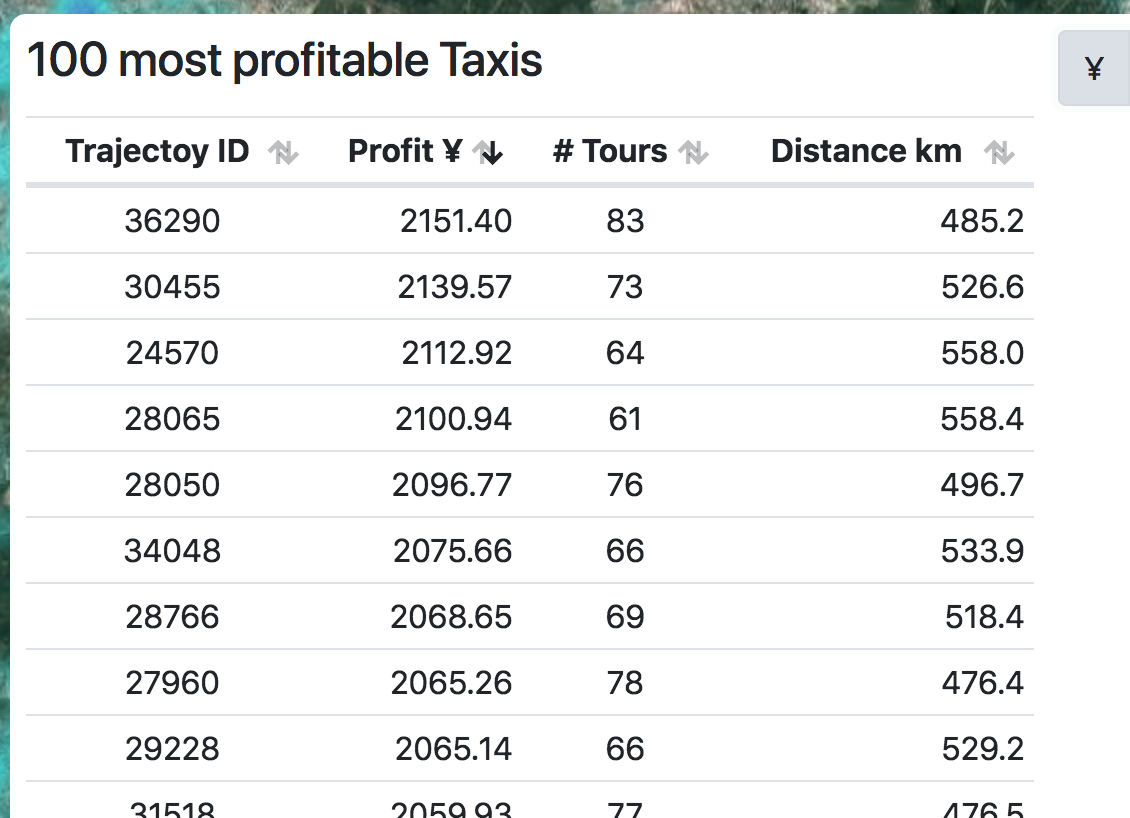
\includegraphics[width=0.5\textwidth]{img/ranking.png}
\caption{Ranking of the most profitable taxis}
\end{figure}


Figure \ref{fig:single_ride} illustrates how the taxi routes are drawn. The line is red if the taxi was driven without a passenger. The line is green if it had a passenger. Arrows indicate the direction. At the end of a tour is always a Yuan symbol on which the user can click. The click lets pop up information about the tour (i.e. start time, end time, distance and the estimated profit).\\

\begin{figure}[h]
\label{fig:single_ride}
\centering
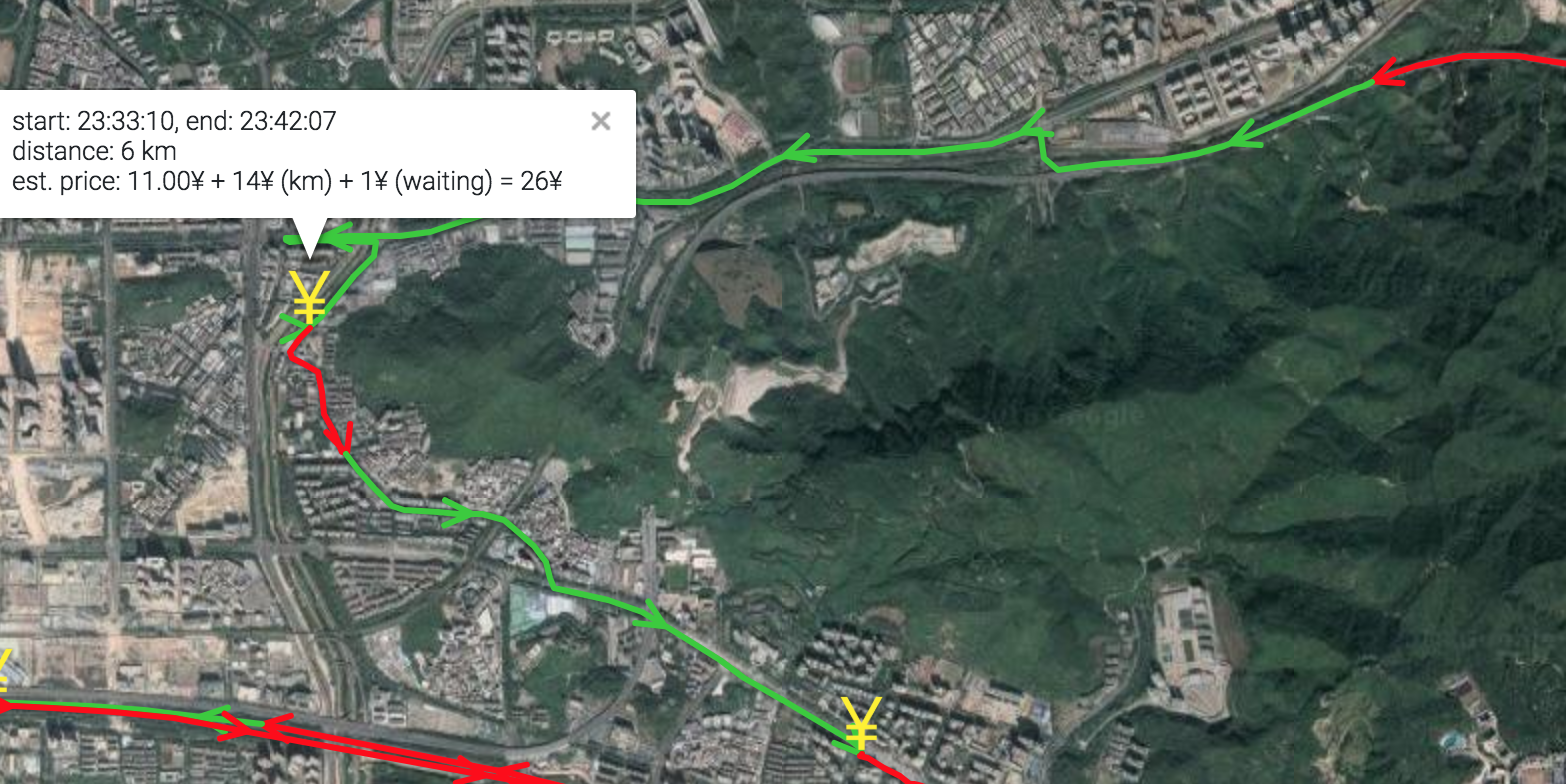
\includegraphics[width=0.5\textwidth]{img/single_ride.png}
\caption{Information about one ride}
\end{figure}

\begin{figure}[h]
\label{fig:best_taxi}
\centering
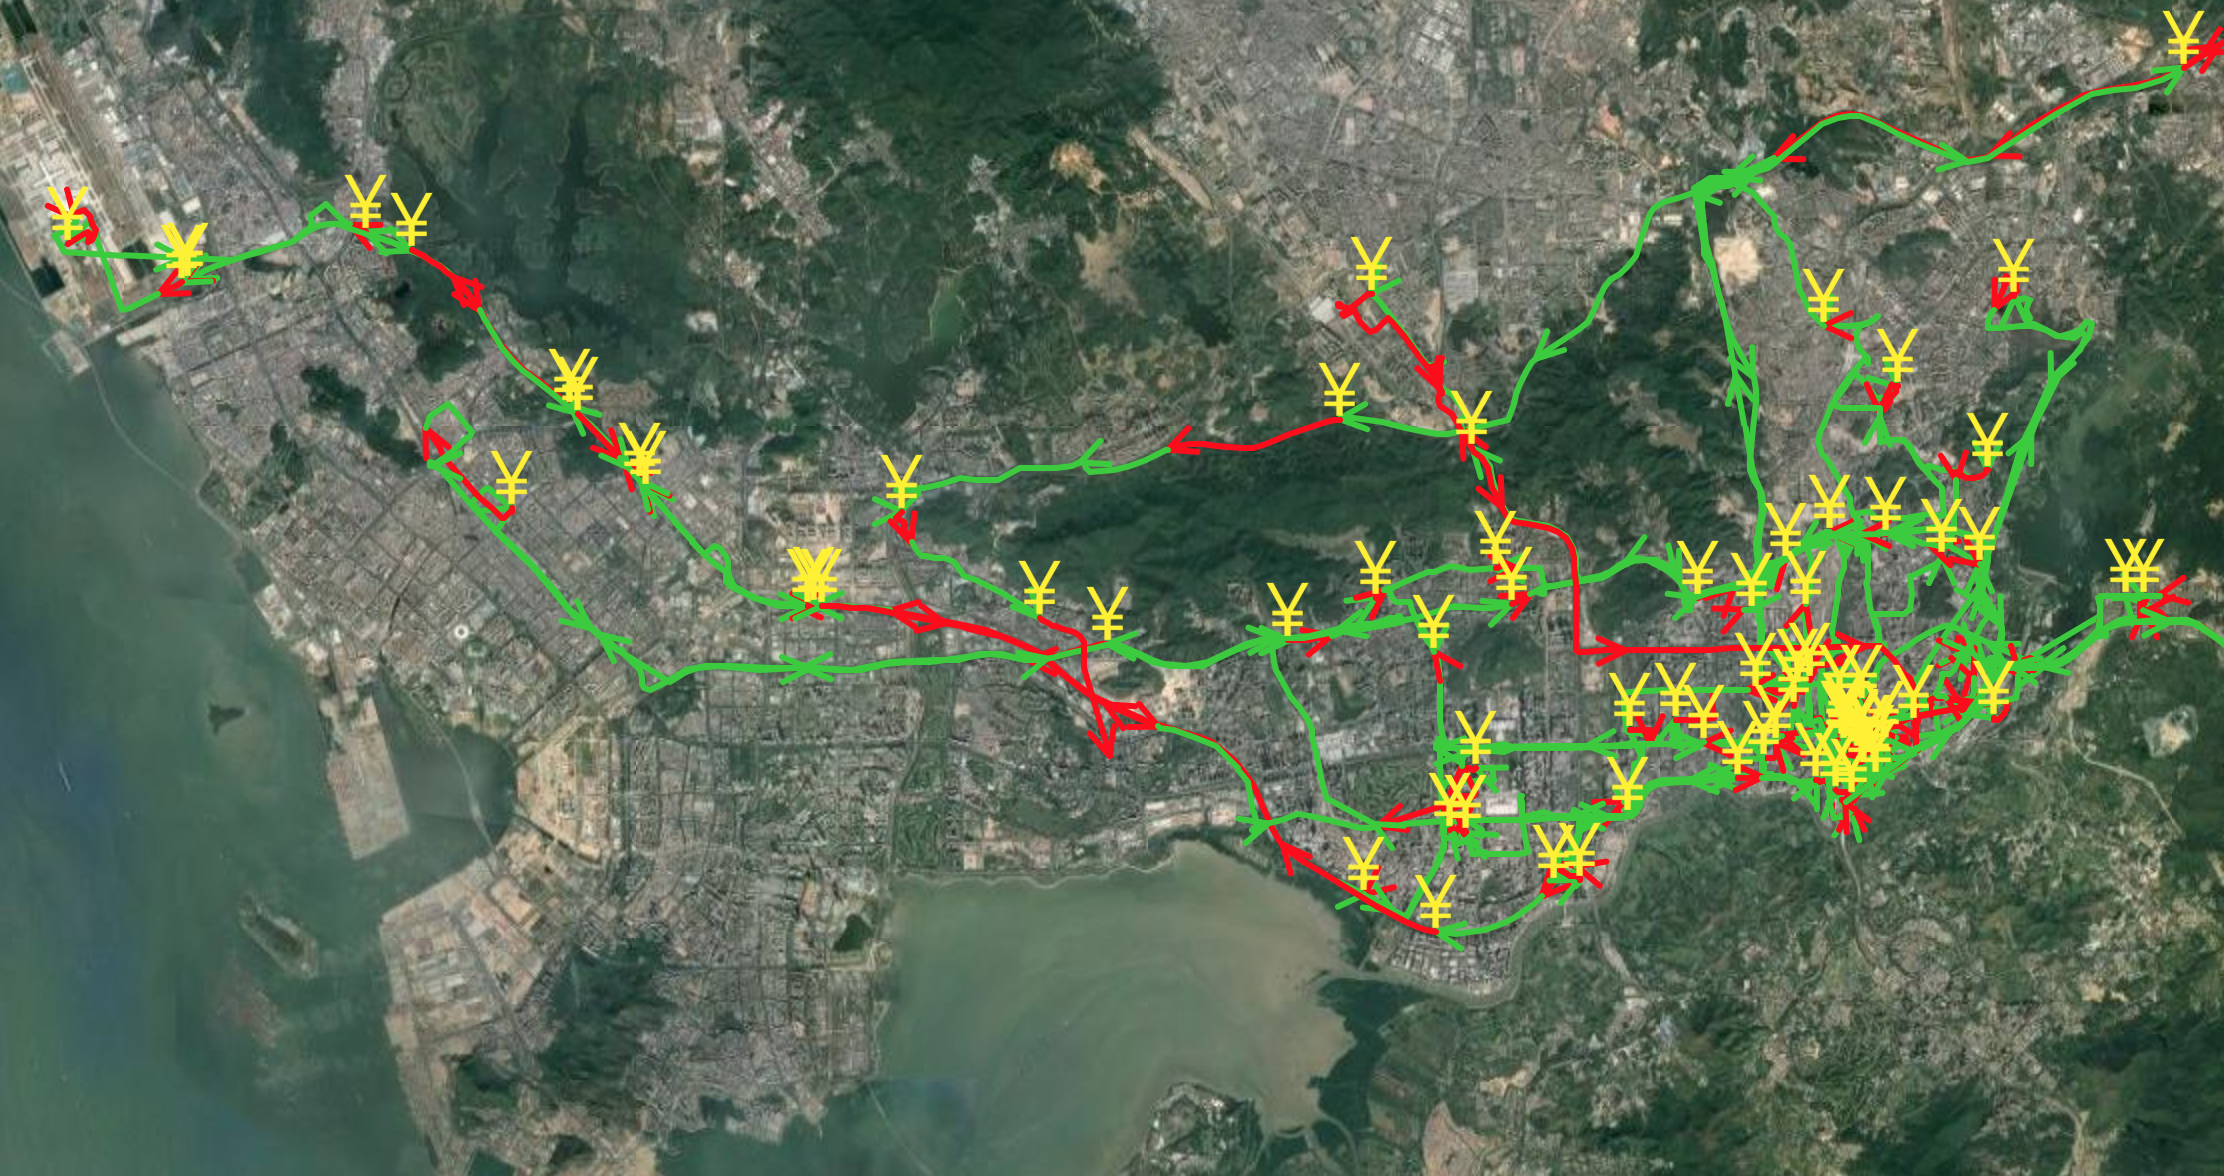
\includegraphics[width=0.5\textwidth]{img/best_taxi.png}
\caption{Entire taxi route}
\end{figure}

\subsection{System Architecture}

\subsection{Data Layouts}

\subsection{Optimizations}

\section{Benchmark Results}

\section{Future Work}

% mehr daten hinzufuegen. kein problem, da alle queries optimiert wurden 

\section{Conclusion}

\section{References}
Generated by bibtex from your ~.bib file.  Run latex,
then bibtex, then latex twice (to resolve references)
to create the ~.bbl file.  Insert that ~.bbl file into
the .tex source file and comment out
the command \texttt{{\char'134}thebibliography}.

\end{document}
